\documentclass[10pt]{article}
\usepackage[breaklinks=true]{hyperref}
\usepackage[margin=0.75in]{geometry}

\usepackage{textcomp}

\usepackage{color}
\usepackage{graphicx}
\definecolor{pblue}{rgb}{0.13,0.13,1}
\definecolor{pgreen}{rgb}{0,0.5,0}
\definecolor{pred}{rgb}{0.9,0,0}
\definecolor{pgrey}{rgb}{0.46,0.45,0.48}

\usepackage{listings}
\lstset{language=bash,
  showspaces=false,
  showtabs=false,
  breaklines=true,
  showstringspaces=false,
  tabsize=2,
  breakatwhitespace=true,
  commentstyle=\color{pgreen},
  keywordstyle=\color{pblue},
  stringstyle=\color{pred},
  numbers=left,
  stepnumber=1,
  basicstyle=\small\ttfamily,
  frame=single,
  moredelim=[il][\textcolor{pgrey}]{$$},
  moredelim=[is][\textcolor{pgrey}]{\%\%}{\%\%}
}

\title{\textbf{Week 09} \\
\Large How Does The Internet Work? Playing with Python3 and cURL}
\author{
	Melvyn Ian Drag
}
\date{\today}


\begin{document}
\maketitle

\begin{abstract}
This Lecture is preamble to the next one in which we will set up an apache webserver. We'll take a peek at Python, revisit cURL, and make some web requests.
\end{abstract}

\section{Goal today}
\begin{itemize}
\item add GET and POST to your vocabulary
\item know that http requests have headers and bodies
\item know how to do GET and POST with curl
\item know how to send data with curl and POST
\item know that Python is whitespace sensitive
\item be able to complete a mildly interesting homework assignment. 
\item know that localhost and 127.0.0.1 are synonyms ( pseudonyms? )
\end{itemize}

\section{Python Webserver}
\subsection{What is Python?}
Python is a scripting language kind of like bash or javascript or perl - but different. It's the favorite language of legions of programmers. Python is used everywhere from scientific computing - I used it to solve PDEs in grad school - to game development, to system administration, to excel spreadsheet modifying, to a million other use cases. Today we're going to look at Python as a language for making websites and serving webpages.

\subsection{What is a webserver?}
As we discussed before, when type a website into a browser ( like Chrome or Firefox, or the like ) and hit \textit{ENTER}, you ask a webserver for some information. The webserver responds with the information you requested and you see a webpage. This type of transaction is called a \textbf{GET} request when performed over the \textbf{Hyper Text Transmission Protocol (HTTP)} or the related \textbf{HTTPS}, which is the secure flavor of HTTP. We'll discuss what we mean by `secure' in a few weeks. 

Another thing you do when talking to a website is give some data to a webserver. This happens when you type your First Name, Last Name, User Name, phone number, password, etc. into a form on a website and click \textit{Submit}. When you click the button, the browser sends a \textbf{POST} request to the webserver that is listening to you from some other corner of the earth. 

In the case of either a GET or POST request, the request goes to a webserver, which is a computer far far away from you that has some code running on it that will respond to your GETs and your POSTs. That code is very often written in Java. It is frequently written in Python. Many write that code in Ruby. Many others use Scala to write the web server code. Recently, people started using Javascript to write the server code. 

In this class we will write the server code in Python.

\subsection{Set up machine}

Install Python3.

\begin{lstlisting}
root@machine$ apt install python3-dev
\end{lstlisting}

Also install a couple of other things, create a new sudoer, and download the class
notes.
\begin{lstlisting}
root@machine$ apt install git curl # we'll need git and curl tonight
root@machine$ adduser yourname
root@machine$ usermod -a -G yourname sudo # or sudo yourname, I can't remember
the order
root@machine$ su - yourname
yourname@machine$ git clone https://github.com/melvyniandrag/LinuxClassRepo.git
\end{lstlisting}

The code we'll use tonight is in the class repo.

\subsection{Don't install Python 2}
Python 2 is being deprecated next year. The Python language maintainers have been telling the Python community to move to Python3 for about 10 years now. If you are new to Python, use Python 3. If you are old to Python, hurry up and port your code to Python 3!

\subsection{I Hate This Lecture Because This is a Linux Class, Not a Python Class}
\textit{Why are you wasting time teaching Python in a Linux class!!!!?!?!? I didn't sign up for this!!}

We're using Python in this class for this webserver activity because I think it is hand's down the easiest language to read and write. Since I don't have time to teach you Python right now, I'm just using Python code because you can more or less skim it and understand what it does. We're only using Python for about the next three hours, so I'm just going to give you  the bare minimum information needed to understand what's happening.

One thing that is important to understand is that Python is a whitespace sensitive language. Whereas other languages use curly braces to denote logical blocks in code - for example, ask class where the \textit{main} and \textit{sayHi} functions , and the \textit{MyClass} class, start and ends in this Java program:
\begin{lstlisting}[language=Java]
public class MyClass{
	public static void sayHi()[
		System.out.println("Hi");
	}

	public static void main(String[] args){
		sayHi();
	}
}
\end{lstlisting}

In python, the situation is different:

\begin{lstlisting}[language=Python]
def sayHi():
	s = "Hi"
	print(s)

if __name__ == "__main__":
	sayHi()
\end{lstlisting}

Note the lack of curly braces. Write this code on your machine and run it as;

\begin{lstlisting}
user@machine$ python3 whateverYouNamedTheFile.py
\end{lstlisting}

Then, change the space before the `s' to 4 spaces and the space before the `print' to a tab. Try to run the code again and it will fail.

 They will look the same, but they are not the same on the byte level. more on that at the end of lecture if there is time. 

Python expects either all tabs or all spaces. If you mix tabs and spaces in your code, Python get's mad.


As I've said before, there is alot of bickering in the tech communty about everything. Some people hate python becuase of the whitespace
\url{https://news.ycombinator.com/item?id=1463451}

I really like Python. I think it's the easiest language to write, there are many great libraries for math, science, system administration, web development, graphics, etc.. The community is great! There are conferences all year long all around the world. And I like not having to wast space in my code with curly braces. Different strokes.

\begin{center}
\textbf{TL;DR You should learn Python. Not now - you're too busy. Next year you should learn Python.}
\end{center}

\subsection{Simple Python Webserver}
Okay, so now that you have Python installed, we can set up a simple web server and begin to make some HTTP GET and SET requests!

Here is the code:
\lstinputlisting[language=Python]{Server.py}

This code is available in the class repository under the name \textit{Server.py}. From just this simple little example, we can learn alot about how the internet works. As we survey the example, we can issue some curl requests and verify that they work.

We can run this code from the command line with:

\begin{lstlisting}
user@machine$ python3 Server.py
Starting httpd server on localhost:8000
\end{lstlisting}

So we see that our little baby website is running on "localhost" at port 8000. Standard HTTP applications run on port 80, but for this demo app we are running on port 8000. Just for reference - HTTPS applications run ( by default ) on port 443. And ssh is over port 22. And postgresql is on port 5432. So now you know 4 special ports!

A summary of what we know about ports so far:
\begin{itemize}
\item port 22 - ssh
\item port 80 - HTTP
\item port 443 - HTTPS
\item port 5432 - PostgreSQL
\end{itemize}

In the webdevelopment world, we make \textbf{GET} and \textbf{POST} requests to webservers that have IP Addresses. But we rarely refer to them by their ip address - typically we use a domain name like `www.google.com' instead of a number address. We are doing the same thing here - we name our local webserver "localhost" instead of referring to it by its numeric name - 127.0.0.1 

\subsection{A quick look at the code} \label{samplehtml}

Note that there are methods for handling \textbf{POST} and \textbf{GET} requests. This is characteristic of code running on a webserver. The code will have methods for handling different types of HTTP requests. You'll also see a few lines of code for setting up an HTTP server to run on `localhost:8000'. Theres a line that does something or other with ``headers", and we'll look into those in a minute. And there's a function that does something with html. If you've never seen HTML before, that's what it looks like. It's a markup language. If you don't know what HTML is, you can learn it in just a few minutes, it's pretty simple. It structures a document between some brackets. HTML always looks something like this:

\begin{lstlisting}[language=HTML]
<html>
<body>
	<h1> This is a title </h1>
	<h2> This is a subtitle </h2>
	<div> This is a paragraph about something </div>
</body>
</html>
\end{lstlisting}

\subsection{Verify Website Works With A Browser}
To verify that our website is running, open a broswer window (chrome, firefox, etc) and type "localhost:8000". You should get a response like this:

\begin{figure}[h]
  \centering
    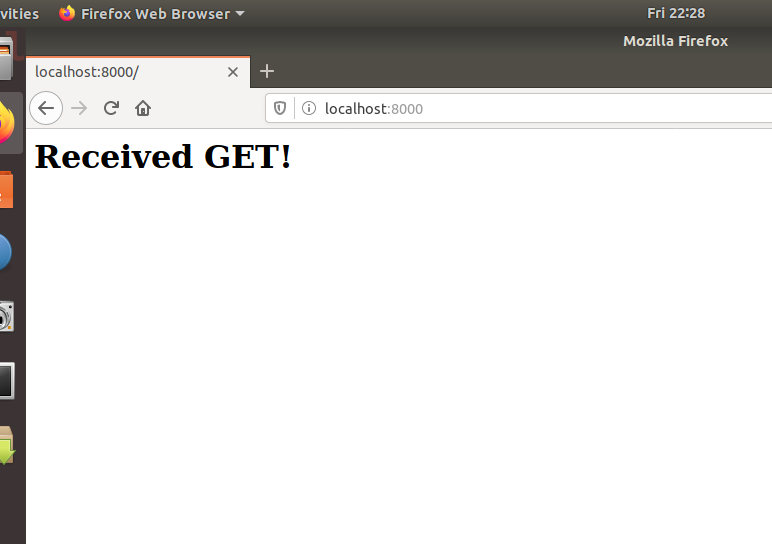
\includegraphics[width=0.5\textwidth]{GET.png}
  \caption{GET request in browser to localhost:8000}
\end{figure}

So we know our website "localhost:8000" is running.

And as I mentioned before, ``localhost" is an alias for ``127.0.0.1", which we can readily verify by going to ``127.0.0.1:8000" while our little application is running.

\begin{figure}[h]
  \centering
    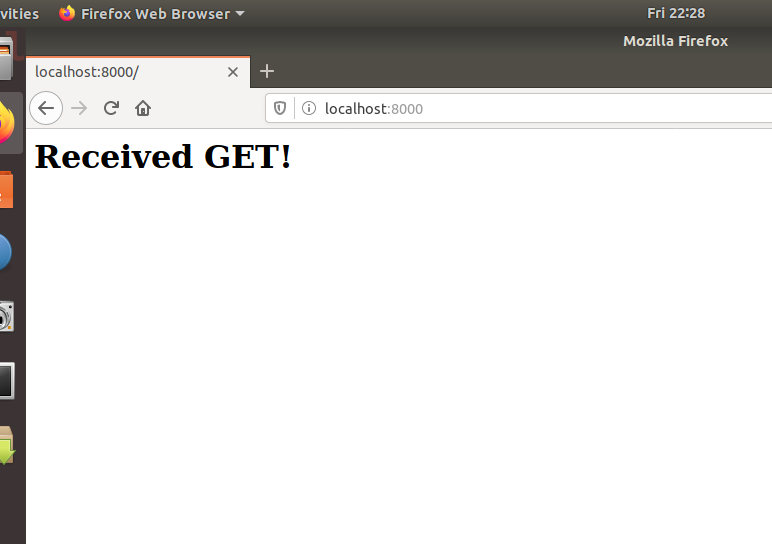
\includegraphics[width=0.5\textwidth]{GET.png}
  \caption{GET request in browser to 127.0.0.1:8000 }
\end{figure}

One more thing of interest - in case you've never seen this happen before - is you can see the Server code handling reqeusts on the server side. Go back to the terminal window where the webserver is running and you'll see it logging output after handling every request.

\begin{figure}[h]
  \centering
    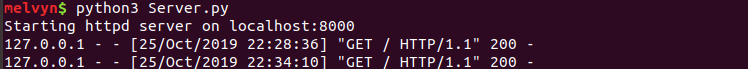
\includegraphics[width=0.5\textwidth]{GET_ServerSide.png}
  \caption{See the webserver handling the GET request traffic. }
\end{figure}

You may be frustrated because something doesn't match up with your expectations here. We see a website in a browser, but how come we don't type ``www.something.com"??? What is this ``localhost" nonsense? What do you mean it's running on port 8000??? I thought you said something or other about port 80 being for http??? All this understanding will come with time. For now we just need to know that websites handle GET and POST requests ( and other types of requests too ). And we've seen a little bit of code that features a get and post handler, and we've verified that ( the GET at least ) works as expected.

Now enough fooling around! Let's use cURL to test out our little website.

\section{Two Exercises}
\begin{center}
\textbf{ \#1 : Change port 8000 in the code to port 80 and try to rerun.}
\end{center}

Some ports are specified for a specific purpose by the os and may require special permissions to use. For example, port 80 requires root access to use. You can try to change the port 8000 in the sample code to port 80 and you will see a permission denied error unless you use sudo.

\begin{figure}[h]
  \centering
    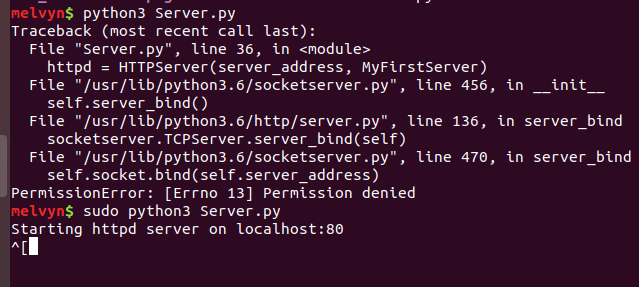
\includegraphics[width=0.5\textwidth]{needRootFor80.png}
  \caption{Need Root Access for Port 80}
\end{figure}


\begin{center}
\textbf{\#2 : Change `localhost' in the code to `127.0.0.1'. Note that is runs as expected - localhost and 127.0.0.1 are the same thing.}
\end{center}

If ip addresses interest you, like, why was `127.0.0.1' selected as `'localhost'? Are there other ip addresses that were designated as local ip addresses? Then you should learn more about computer networking! I admit that I'm very interested in the subject, but haven't studied it enough due to other responsibities and ambitions.


\section{10 Minute Break}
We'll take a 10 minute break now in case you need a coffee or to go to the bathroom. If you don't mind continuing to work, I encourage you to change the GET request in your little website so that your browser displays the HTML from section \ref{samplehtml}. If you can do that, try to modify it some more with some other HTML tags.

\section{cURL}
cURL is a Linux tool that has been around for about 20 years. It's used for making requests. It can be thought of as a command line browser, in some sense. The things you usually do  in a browser, like typing an address into a search bar, entering data into a form on a web page, clicking a button - these things can be done on the command line with cURL ( mostly ).

\subsection{Exercise \#1}
Open another terminal window in addition to the one running your Python webserver. Then enter these commands:

\begin{lstlisting}
user@machine$ curl localhost:8000
# returns some html from the website
user@machine$ curl -X GET localhost:8000
# returns the same thing, because the default curl action is GET
user@machine$ curl -X POST -d"myname=melvyn" localhost:8000
# returns the POST response, along with the data you passed in
user@machine$ curl -X POST --verbose -d"myname=melvyn" localhost:8000
# returns the same thing, but this time with lots of extra information!
# this time you can see what you sent over via the POST in detail
# along with a detailed response from the server
# The lines with a > are what you sent.
# The lines with a < are what came back.
user@machine$ curl -X POST --verbose -d"myname=melvyn&mylastname=drag" localhost:8000
# Try sending more and more data values by separating them with an ampersand.
user@machine$ curl -X POST -H "Content-Type: application/text" -H "Content-Length: 10" -d"myname=melvyn" localhost:8000
# Look what happened due to Content-Length, play around with the length to see what else happens
# also check and see if anything happens if you change Content-Type to application/json or application/x-www-form-urlencoded
user@machine$
\end{lstlisting}

The `-X' flag is used for specifying the HTTP verb associated with your request. As you've seen, the webserver will contain code for handling different types of requests.

The `-d' flag is used for passing data. Typically we associate the `-d' flag with POST requests and not GET requests.

\subsection{Headers}
As with most other data transmission protocols, file formats, etc. - most computer data formats - there is a header, followed by a body. Whenever you send an HTTP request, some header data goes along with it. Two of the more common ones you'll see are:

\begin{enumerate}
\item Content-Length - how long the data being passed is
\item Content-Type - what type of data is being sent? Json? Text? HTML? Other?
\end{enumerate} 


\subsection{HTTP Return Codes}
There are many different return codes. When you send a request to a webserver, it responds with some header data, a body, and also, a return code. Common return codes that you may have seen already are:

\begin{enumerate}
\item 200 (OK) - The 200 return code is when you HTTP transaction succeeds
\item 404 (Not Found) - Happens when you request something from the internet that is not there
\item 500 ( Internal Server Error ) - Generic message for when something has gone wrong with the server
\end{enumerate}

To see a 200, type
\begin{lstlisting}
curl --verbose https://www.google.com  2>&1 | grep "^< HTTP"
\end{lstlisting}

To see a 404 type
\begin{lstlisting}
icurl --verbose https://www.google.com/doesntExist  2>&1 | grep "^< HTTP"
\end{lstlisting}

To see a 500 - I'm not sure how to force this error off the top of my head.

More information about return codes can be found here:
\url{https://en.wikipedia.org/wiki/List_of_HTTP_status_codes}

I said I'm not sure how to force the 500 error because I'm not an experience web programmer - but I do know a thing or two about Linux. Did you all understnad the piped commands I used to generate the status codes?

Two interesting things:

\begin{itemize}
\item 2\textgreater\&1 means pass stderr to stdout. Did this because curl seems to dump to stderr.
\item grep ``\^\textless HTTP" means find a line starting with ``\textless HTTP"
\end{itemize}

\subsection{Congratulations!}
You may have just run your first webserver! If this wasn't your first webserver project, I hope it was fun anyway.

As I said, the purpose of this assignment is not for you to become a webdeveloper, but just for you to know a couple of things so that when we set up an Apache webserver, it's not totally foreign to you.

\section{A Real World Curl Example}
Let's do a real world curl example right now. You may want to use curl to make a web request.

To illustrate what we are going to do now, see the following two images:

\begin{figure}[h]
  \centering
    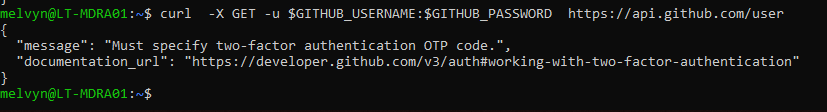
\includegraphics[width=0.9\textwidth]{unsuccessfulGithubAPIHit.png}
  \caption{Couldn't access api}
\end{figure}

\begin{figure}[h]
  \centering
    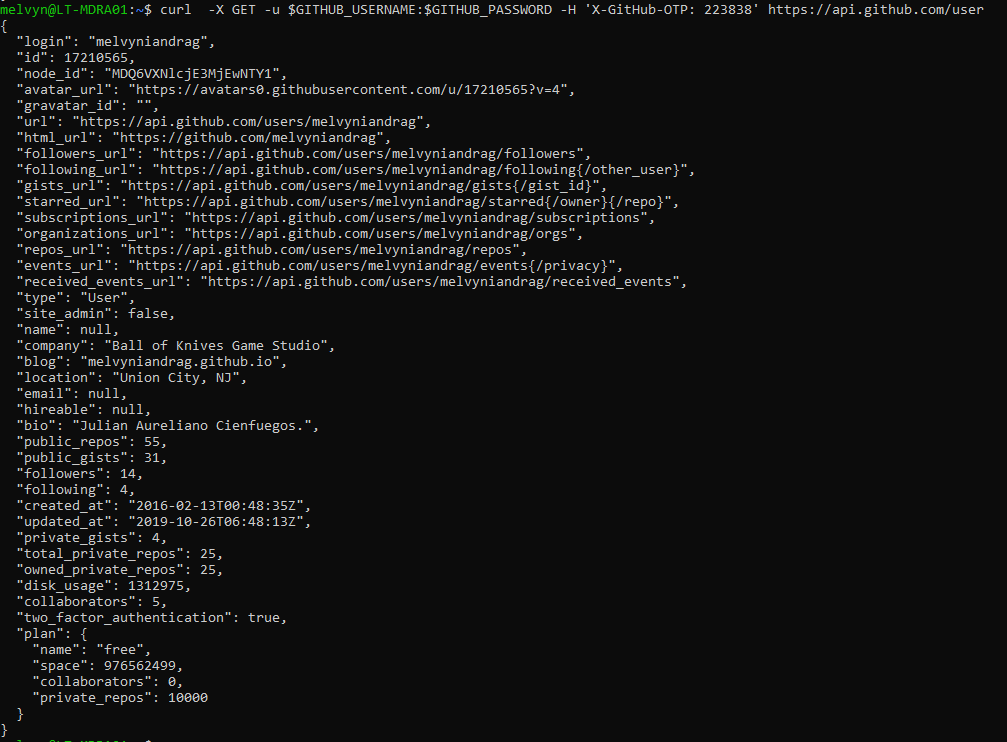
\includegraphics[width=0.9\textwidth]{successfulGithubAPIHit.png}
  \caption{Could access api}
\end{figure}


\begin{enumerate}
\item Have everyone turn on 2fA on their github accounts
\item In \texttildelow/.bashrc add the line `export GITHUB\_USERNAME=yourusername'
\item In \texttildelow/.bashrc add the line `export GITHUB\_PASSWORD=yourpassword'
\item Don't let anyone see this!
\item source \texttildelow/.bashrc
\item Now we are ready
\end{enumerate}

How to request a 2FA code be sent to your phone
\begin{lstlisting}
 curl -X POST \
	-u $GITHUB_USERNAME:$GITHUB_PASSWORD \
	-H 'Content-Type: application/json' \
	-d '{"scopes": ["user:email"],"note": "blog example"}' \
	https://api.github.com/authorizations
\end{lstlisting}

How to use it
\begin{lstlisting}
curl  -X GET \
	-u $GITHUB_USERNAME:$GITHUB_PASSWORD \
	-H 'X-GitHub-OTP: 223838' \
	https://api.github.com/user
\end{lstlisting}


Note that in this example, we could omit the -X GET, because that is the default behavior.

Note that there are different ways to supply parameters to cURL - I can put --header instead of -H

\begin{lstlisting}
curl  -X GET \
	-u $GITHUB_USERNAME:$GITHUB_PASSWORD \
	--header 'X-GitHub-OTP: 884813'
	 https://api.github.com/user
\end{lstlisting}

\subsection{Exercise}
Have students create a private gist on github and query github with curl to see the number of their private gists go up.

\subsection{Another exercise}
Create a private repo on github. See that you can download a file from it using the REST API. Add just a readme to the private repo.

Prompt github to send you a 2fa key.Then get the readme like this:

\begin{lstlisting}
curl  -X GET \
	-u $GITHUB_USERNAME:$GITHUB_PASSWORD \
	-H 'X-GitHub-OTP: 413096' \
	https://api.github.com/repos/melvyniandrag/IntroToJavaFall2019/contents/Readme.md
\end{lstlisting}

( but make sure to set the code to the one given to you by github via the phone or email, however they send you the 2FA code. )

Note that the encoding is something calle "base64".  There are many encodings out there. In my JAva class we talked quite a bit about Hex, binary, and decimal encodings for bytes. Then for text we talked about encodings like ASCII, UTF8 and UTF16. We'll visit those topics in this class eventually, but for now it's just something interesting to look at.You'll see that the content of your Readme.md file is NOT what you put on github - its a bunch of random alphanumeric cahracters in something called "base64". Interesting! But what does it mean?!>! You'll have to wait and see! Unless your curiosity gets the better of you, in which case you can just go online and loo kup what base64 encoding is.

\begin{figure}[h]
  \centering
    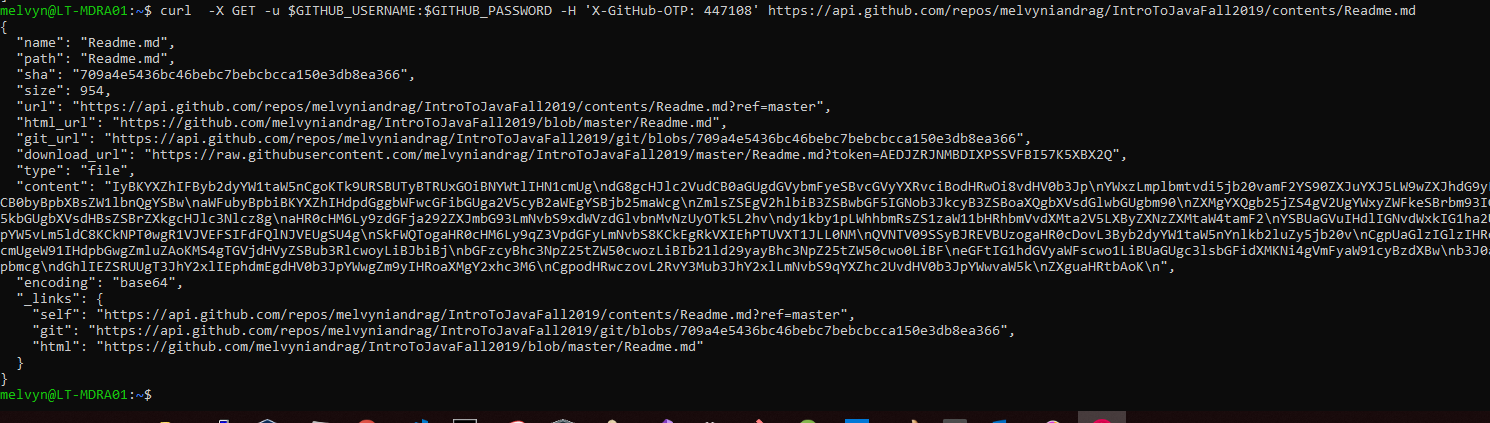
\includegraphics[width=0.9\textwidth]{getReadme.PNG}
  \caption{See how I got the readme data}
\end{figure}

\subsection{Danger of curl in place of 2FA}
There was a security leak a little while back at paypal whereby you could bypass 2FA using curl.
\url{https://duo.com/blog/duo-security-researchers-uncover-bypass-of-paypal-s-two-factor-authentication}

\subsection{See these references}
\url{https://developer.github.com/v3/auth/#working-with-two-factor-authentication}
\url{https://blogs.infosupport.com/accessing-githubs-rest-api-with-curl/}

\section{What's a REST API}
There are just too many buzzwords out there. I've showed you that we could get html back with curl when we curled out own little python server. Then I showed you that when we curled api.github.com, we got back JSON data. There is more to it, but in general, when we send and receive JSON, we call this a REST API. If you look into web development more, you'll  learn what the REST stand for, and then you'll learn why RESTful ness is important. For us it doesn't matter at all. All that matters is that you can see that REST is for exchanging JSON data.

\subsection{Job interview prep}
\noindent\textit{\textbf{Interviewer:} I see you know a bit about Linux webserver maintenance. Do you know what a REST API is?}

\noindent \textbf{You: } Honestly, not too much because I'm not a webdeveloper. But I do know that REST APIs are very popular now, and they typically involve the exchange of JSON data. JSON data is when the data is structured like a Python dicitonary, or a Java Hashmap  - its a bunch of key-value pairs in curly braces.

If you can give the above answer, you'll know enough for now.

\section{Back to Tabs and Spaces}
We briefly mentioned the difference between tabs and spaces. You can set the tab width in Vim. Maybe mention the ASCII codes for tab vs space so that the folks in the Java class can make the connection.

\section{Recap of what you know}
\begin{enumerate}
\item A bit about the Bash programming language
\item grep \& regular expressions
\item What a user is on Linux
\item What a group is on Linux
\item What is git?
\item You're comfortable using a command line interface now
\item There are a few different languages on the command line - we've used bash and dash
\item What permissions are and how to modify them
\item What is a root user
\item What is a process
\item What is a job
\item How to send signals to processes ( kill, CTRL+C, CTRL+Z )
\item How to make code ignore or block signals
\item How to install software on Linux
\item A cool trick for using setuid / setgid to make a non-root user do some root stuff
\item basics of relational dbs and how to configure one on Linux
\item What is cron
\item curl
\item some vocabulary like API, REST, regex, SQL, DB
\item A bit about python programming
\end{enumerate}

\section{Coming Up In This Class}

We have a few more important things to cover
\begin{enumerate}
\item set up apache webserver
\item set up a git server
\item add a gitlab front end to the git server
\item Linux and Text encodings
\item xxd, everyone's favorite binary packet analyzer
\item The AWK programming language
\item The hows and whys of formatting harddrives, usb sticks, solid state drives, etc.
\item Encryption with gpg + pgp. How it relates to ssh and other pub/priv key schemes.
\item sed
\end{enumerate}

\end{document}
